\documentclass[tikz,border=2pt]{standalone}
\usepackage{amsmath,amssymb}
\usepackage{tikz}
\usetikzlibrary{arrows.meta}

\begin{document}
% The arrival rate lambda is the slope of the expected count: E[N_t] = lambda t. A single
% realisation (staircase) fluctuates around that line; here lambda = 0.8 per unit time.
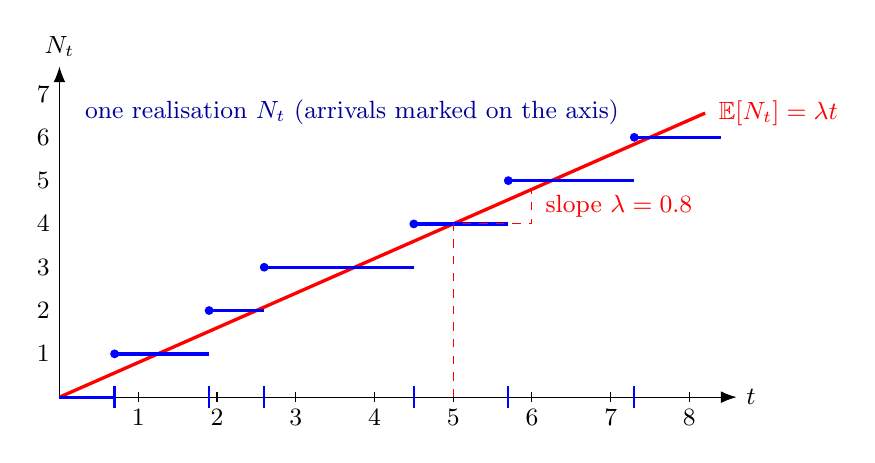
\begin{tikzpicture}[every node/.style={font=\small}, >={Latex[length=2mm]}]
	\draw[->] (0,0) -- (8.6,0) node[right] {$t$};
	\draw[->] (0,0) -- (0,4.2) node[above] {$N_t$};
	\foreach \t in {1,...,8} {\draw (\t,0.06) -- (\t,-0.06); \node[below=1pt, font=\small] at (\t,0) {\t};}
	\foreach \y in {1,...,7} {\node[left, font=\small] at (0,{\y*0.55}) {\y};}
	\draw[red, very thick] (0,0) -- (8.2,{8.2*0.8*0.55});
	\node[red, anchor=west, font=\small] at (8.25,{8.2*0.8*0.55}) {$\mathbb{E}[N_t]=\lambda t$};
	\draw[blue, very thick] (0,0) -- (0.7,0) (0.7,0.55) -- (1.9,0.55) (1.9,1.1) -- (2.6,1.1) (2.6,1.65) -- (4.5,1.65) (4.5,2.2) -- (5.7,2.2) (5.7,2.75) -- (7.3,2.75) (7.3,3.3) -- (8.4,3.3);
	\foreach \t/\y in {0.7/0.55, 1.9/1.1, 2.6/1.65, 4.5/2.2, 5.7/2.75, 7.3/3.3} {\fill[blue] (\t,\y) circle (1.6pt); \draw[blue, thick] (\t,-0.14) -- (\t,0.14);}
	\draw[red, dashed] (5,0) -- (5,2.2) -- (6,2.2) -- (6,2.64);
	\node[red, font=\small, anchor=west] at (6.05,2.42) {slope $\lambda=0.8$};
	\node[blue!60!black, font=\small, anchor=north west] at (0.2,3.9) {one realisation $N_t$ (arrivals marked on the axis)};
	
\end{tikzpicture}
\end{document}
